\documentclass[]{article}
\usepackage{lmodern}
\usepackage{amssymb,amsmath}
\usepackage{ifxetex,ifluatex}
\usepackage{fixltx2e} % provides \textsubscript
\ifnum 0\ifxetex 1\fi\ifluatex 1\fi=0 % if pdftex
  \usepackage[T1]{fontenc}
  \usepackage[utf8]{inputenc}
\else % if luatex or xelatex
  \ifxetex
    \usepackage{mathspec}
  \else
    \usepackage{fontspec}
  \fi
  \defaultfontfeatures{Ligatures=TeX,Scale=MatchLowercase}
\fi
% use upquote if available, for straight quotes in verbatim environments
\IfFileExists{upquote.sty}{\usepackage{upquote}}{}
% use microtype if available
\IfFileExists{microtype.sty}{%
\usepackage{microtype}
\UseMicrotypeSet[protrusion]{basicmath} % disable protrusion for tt fonts
}{}
\usepackage[top=3cm,left=3cm,right=3cm]{geometry}
\usepackage{hyperref}
\hypersetup{unicode=true,
            pdftitle={Disease Modeling Results},
            pdfborder={0 0 0},
            breaklinks=true}
\urlstyle{same}  % don't use monospace font for urls
\usepackage{longtable,booktabs}
\usepackage{graphicx,grffile}
\makeatletter
\def\maxwidth{\ifdim\Gin@nat@width>\linewidth\linewidth\else\Gin@nat@width\fi}
\def\maxheight{\ifdim\Gin@nat@height>\textheight\textheight\else\Gin@nat@height\fi}
\makeatother
% Scale images if necessary, so that they will not overflow the page
% margins by default, and it is still possible to overwrite the defaults
% using explicit options in \includegraphics[width, height, ...]{}
\setkeys{Gin}{width=\maxwidth,height=\maxheight,keepaspectratio}
\IfFileExists{parskip.sty}{%
\usepackage{parskip}
}{% else
\setlength{\parindent}{0pt}
\setlength{\parskip}{6pt plus 2pt minus 1pt}
}
\setlength{\emergencystretch}{3em}  % prevent overfull lines
\providecommand{\tightlist}{%
  \setlength{\itemsep}{0pt}\setlength{\parskip}{0pt}}
\setcounter{secnumdepth}{5}
% Redefines (sub)paragraphs to behave more like sections
\ifx\paragraph\undefined\else
\let\oldparagraph\paragraph
\renewcommand{\paragraph}[1]{\oldparagraph{#1}\mbox{}}
\fi
\ifx\subparagraph\undefined\else
\let\oldsubparagraph\subparagraph
\renewcommand{\subparagraph}[1]{\oldsubparagraph{#1}\mbox{}}
\fi

%%% Use protect on footnotes to avoid problems with footnotes in titles
\let\rmarkdownfootnote\footnote%
\def\footnote{\protect\rmarkdownfootnote}

%%% Change title format to be more compact
\usepackage{titling}

% Create subtitle command for use in maketitle
\providecommand{\subtitle}[1]{
  \posttitle{
    \begin{center}\large#1\end{center}
    }
}

\setlength{\droptitle}{-2em}

  \title{Disease Modeling Results}
    \pretitle{\vspace{\droptitle}\centering\huge}
  \posttitle{\par}
    \author{}
    \preauthor{}\postauthor{}
    \date{}
    \predate{}\postdate{}
  
\usepackage{multirow}
\usepackage{multicol}
\usepackage{booktabs}
\usepackage{xcolor}
\numberwithin{equation}{section}
\counterwithin{figure}{section}
\counterwithin{table}{section}
\usepackage{dcolumn}
\usepackage{rotating}
\usepackage{caption}
\usepackage{amsfonts}
\captionsetup{width=4.5in}
\usepackage{algorithm}

\begin{document}
\maketitle

{
\setcounter{tocdepth}{2}
\tableofcontents
}
\hypertarget{results}{%
\section{Results}\label{results}}

In this paper, I have implemented an MCMC algorithm that estimates the
Two-Component Model from simulated data. The simulation parameters are
taken from ({\textbf{???}})

\begin{longtable}[]{@{}cc@{}}
\toprule
parameters & simulation values\tabularnewline
\midrule
\endhead
K: number of changespoints & 2\tabularnewline
\(\boldsymbol{\lambda}\): epidemic parameters & 0.7, 1.2,
0.7\tabularnewline
\(\boldsymbol{\gamma}\): endemic parameters & log(10), 0.5,
1.5\tabularnewline
\(\boldsymbol{\theta}\): changepoints & 39, 49\tabularnewline
\bottomrule
\end{longtable}

\begin{figure}
\centering
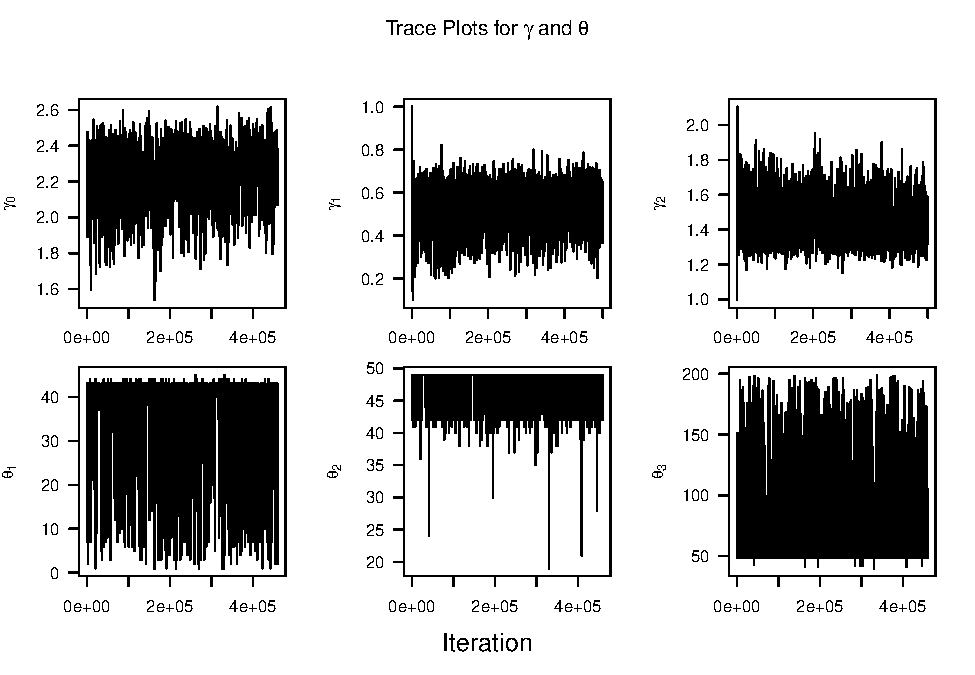
\includegraphics{thesis_results_section_files/figure-latex/unnamed-chunk-1-1.pdf}
\caption{mycaption}
\end{figure}

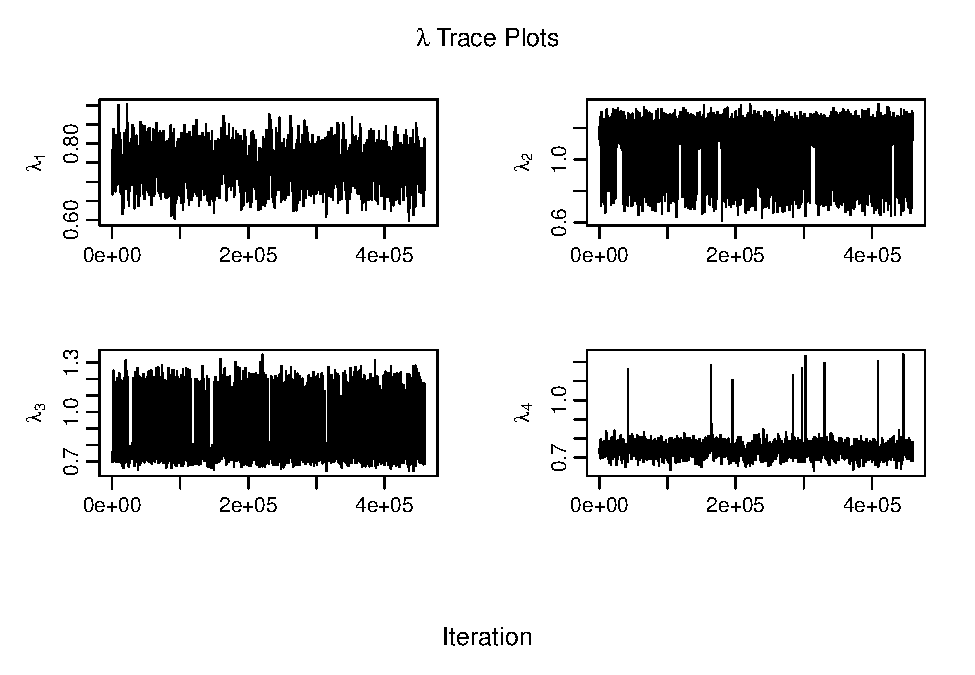
\includegraphics{thesis_results_section_files/figure-latex/lambda_traces-1.pdf}

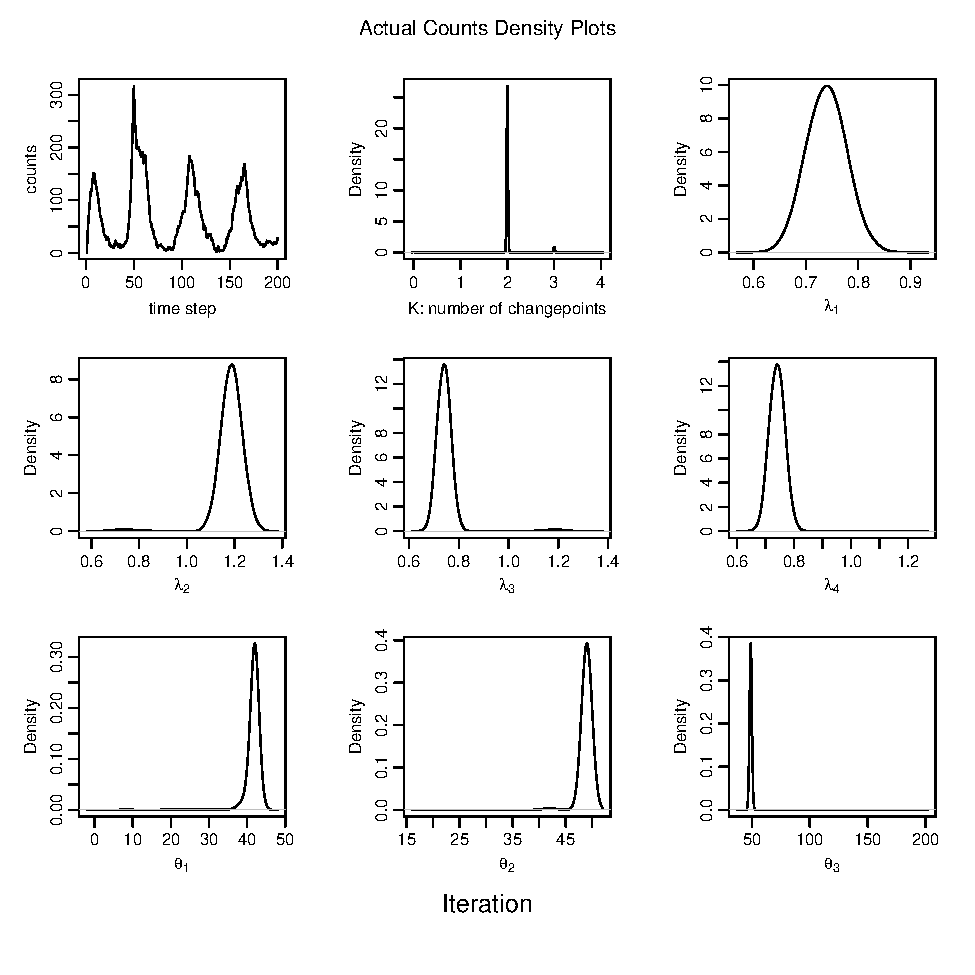
\includegraphics{thesis_results_section_files/figure-latex/density_plots-1.pdf}

\hypertarget{two-component-model-on-simulated-data}{%
\subsection{Two-Component Model on Simulated
Data}\label{two-component-model-on-simulated-data}}

Beginning with the simple

\hypertarget{graph-estimation-on-fixed-two-component-model}{%
\subsection{Graph Estimation on Fixed Two-Component
Model}\label{graph-estimation-on-fixed-two-component-model}}

\hypertarget{conclusiondiscussion}{%
\section{Conclusion/Discussion}\label{conclusiondiscussion}}

\hypertarget{citations}{%
\section{Citations}\label{citations}}


\end{document}
